\section{Введение}
    Вводный текст с описанием задачи и схемы.
    \begin{figure}[H]
        \centering
        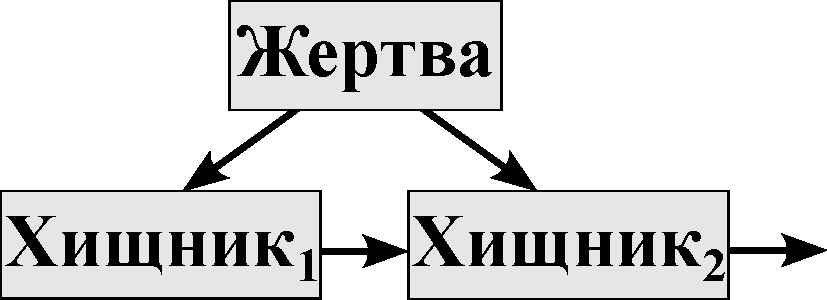
\includegraphics[width=10cm]{pictures/scheme.pdf}
    \end{figure}


\pagebreak

\section{Математический аппарат}
    \subsection{Методы анализа}
    Исследуемые далее модели конкуренции представляют собой автономные системы трёх дифференциальных уравнений.
    \[
        \dot{x} = f(x), \quad x = (x_1, x_2, x_3).
    \]

    Для данных систем будет проведён анализ точек равновесия:
    \[
        \dot{x} = 0 \Rightarrow f(x) = 0
    \]

    Для каждой точки равновесия (\( x^* \) -- решение данной однородной системы уравнений) будет проведён анализ по методу первого приближения\cite{filipov}.

    В матрицу Якоби данной системы \( \left( \frac{\partial f}{\partial x} \right) \) нужно подставить точку равновесия. После чего нужно найти собственные значения этой матрицы:
    \[
        \det \left( \lambda I - \frac{\partial f}{\partial x}\big|_{x^*} \right) = 0 ~ \Rightarrow ~ b_0 \lambda^3 + b_1 \lambda^2 + b_2 \lambda + b_3 = 0.
    \]

    Для того, чтобы точка была устойчивой, необходимо, чтобы \( \forall i \, \Rez \lambda_i < 0 \). Однако, напрямую решать кубическое уравнение может быть непросто, поэтому можно воспользоваться критерием Рауса-Гурвица\cite{nefedov}. Для этого построим матрицу Гурвица: 
    \[
        \Delta = \left( \begin{matrix}
            b_1 & b_3 & 0 \\
            b_0 & b_2 & 0 \\
            0   & b_1 & b_3
        \end{matrix} \right)
    \]
    Если \( b_0 > 0\), то для устойчивости необходимо, чтобы все главные миноры матрицы \( \Delta \) были положительны:
    \[
        \begin{split}
            & \Delta_1 = b_1, \\
            & \Delta_2 = b_1 b_2 - b_3 b_0, \\
            & \Delta_3 = b_3 \Delta_2.
        \end{split}
    \]

    \subsection{Численные методы}
    Для получения численных решений системы дифференциальный уравнений будет использоваться метод Рунге-Кутты 4 порядка\cite{berez}.

    Для программной реализации используется язык Python с библиотеками numpy и matplotlib.